\subsection{Prior Predictive Distribution for $\tilde{\mu}^a$}
Here, we study the prior predictive distribution of $\tilde{\mu}^a$, the underlying 'true' value of the parameter $a$ for a patient with covariate vector $\tilde{x}$.  The goal of this section is to see how our prior belief on what $\tilde{\mu}^a$ varies depends on the hyperparameters.  We first claim that in the prior predictive distribution, $\tilde{\mu}^a$ follows a logit-normal distribution, whose properties we will now describe.

\subsection{Logit-Normal Distribution}
A logit-normal distribution is a continuous distribution defined on the open interval $(0,1)$.  A random variable $X$ follows a logit-normal distribution if the transformed random variable $\textrm{logit}(X)$ follows a normal distribution.  An equivalent definition makes the parameterization of a logit-normal distribution clear:
\begin{defn}
If $Y \sim \textrm{Normal}(\mu, \sigma)$ , then the transformed random variable $X=\textrm{logistic}(Y)$ follows a $\textrm{Logit-Normal}(\mu, \sigma)$ distribution. 
\end{defn}

Thus, a Logit-Normal distributed random variable $X$ is parameterized using the mean and standard deviation of the normal distribution that $\textrm{Logit}(X)$ follows.

\subsubsection{Key Properties}

Applying the change of variable formula to the density function of a $\textrm{Normal}(\mu, \sigma)$ random variable under the logistic transformation, one arrives at the density function of a $\textrm{Logit-Normal}(\mu, \sigma)$ random variable:

\begin{eqnarray}
f_X(x;\mu, \sigma) = \frac{1}{\sigma \sqrt{2\pi}} \exp{-\frac{(\textrm{logit}(x) - \mu)^2}{2 \sigma^2}}\frac{1}{x(1-x)};   x \in (0,1)
\end{eqnarray}

Unfortunately, there are no analytical formulas for the mean, variance, or mode of a logit-normal distribution.  

\subsubsection{Unimodality}

In general, the density of a logit-normal distribution may have either $1$ or $2$ modes.  For sufficiently large $\sigma$, a $\textrm{Logit-Normal}(\mu, \sigma)$ distribution will have 2 modes - one near 0 and one near 1.  This intuitively makes sense, because a sufficiently diffuse normal distribution will have significant mass far away from 0, where the slope of the logistic function is nearly flat.  Conversely, for sufficiently small $\sigma$, $f_X(x;\mu,\sigma)$ will be unimodal.  This result can be seen analytically.

By taking the derivative of $f_X(x; \mu, \sigma)$, it can be seen that the modes of $f_X(x;\mu, \sigma)$ occur at $x$ for which the following condition is satisfied:

\begin{eqnarray}
\textrm{logit}(x) = \sigma^2(2x-1) + \mu
\end{eqnarray}

For any $\mu$ and $\sigma$, there is always at least 1 $x$ for which this condition is satisfied.  Thus, $f_X(x;\mu, \sigma)$ always has at least 1 mode.  Furthermore, as the slope of $\textrm{logit}(x)$ is always greater than 1, we see that if $\sigma^2 < 1$, there is exactly 1 $x$ such that the condition is satisfied, and arrive at the following observation:

\begin{obs}
If $\sigma^2 \leq 1$, then $f_X(x;\mu, \sigma)$ is unimodal.
\end{obs}

\subsection{Logit-Normality of $\tilde{\mu}^a$ in the Prior}
The only hyperparameter that $\tilde{\mu}^a$ depends on in the prior is $\Sigma^a=c^aI$.  Now, we see that $\tilde{\mu}^a|c^a$, the prior predictive distribution of $\mu^a$, follows the logit-normal distribution.  This is because $B^a \sim N(0, \Sigma^a)$ and so $B^a\tilde{x} \sim N(0, \tilde{x}'\Sigma^a\tilde{x})$.  Then, $\mu_{pop}^{a*} + B^a\tilde{x} \sim N(\mu_{pop}^{a*}, \tilde{x}'\Sigma^a\tilde{x})$.  Finally, as $\tilde{\mu^a}|c^a \sim g^a(\mu_{pop}^{a*} + B^a\tilde{x})$ and $g^a$ was defined to be the logistic function, we arrive at the following observation:

\begin{obs}
  $\tilde{\mu}^a|c^a \sim \textrm{Logit-Normal}(\mu_{pop}^{a*},  \tilde{\sigma}^a)$, where $\tilde{\sigma}^a$ $=$ $\tilde{x}'\Sigma^a\tilde{x} = c^a\sum_{j=1}^k \tilde{x}_j^2$
\end{obs}

where we have used the fact that $\Sigma^a$ was parameterized by the hyperparameter $c^a$.

\subsection{Dependence of Prior Predictive Distribution of $\tilde{\mu}^a$ on Hyperparameters}

For a test sample $\tilde{x}$, the prior predictive distribution $\tilde{\mu}^a|c^a$ is distributed $\textrm{Logit-Normal}(\mu_{pop}^{a*}, \tilde{\sigma}^a)$, where $\mu_{pop}^{a*} = g^a(\mu_{pop}^{a})$ and $\tilde{\sigma}^a$ is as defined in the previous section.  Let us first see how this prior predictive distribution depends on $\mu_{pop}^{a}$ and $\tilde{\sigma}^a$.  In Figure X, we have plotted for several values of $\mu_{pop}^{a}$, how the prior predictive distribution $\tilde{\mu}^a|c^a$ depends on $\tilde{\sigma}^a$.  The vertical line denotes the location of $\mu_{pop}^{a}$.

There are several things to note from the figure:
\begin{enumerate}
\item As $\tilde{\sigma}^a$ approaches 0, $\textrm{Logit-Normal}(\mu_{pop}^{a*}, \tilde{\sigma}^a)$ converges to the point mass at $\mu_{pop}^{a}$.  Recall that we are normalizing the covariate vectors so that each covariate has mean 0 and standard deviation 1 over the training data, so that if a test sample $\tilde{x}$ is equal to the 'average' patient of the training data, then $\tilde{x} = 0$.  This means that the more similar a test sample $\tilde{x}$ is to the 'average' patient, the more closer $\tilde{x}$ is to 0, the smaller $\tilde{\sigma}^a$ is, and thus the more strongly we believe in the prior that $\tilde{\mu}^a$ is equal to $\mu_{pop}^{a}$, the average of $a$ in the training data.  This is what we want.
\item If $\tilde{\sigma}^a \leq 1$, then $P(\tilde{\mu}^a;c^a)$ is necessarily unimodal.  If $\tilde{\sigma}^a > 1$, then $f(\tilde{\mu}^a;c^a)$ might still be unimodal, but not necessarily.
\item As $\tilde{\sigma}^a$ increases, the mode of $P(\tilde{\mu}^a;c^a)$ increases.  While we would like the mode to remain constant as $\tilde{\sigma}^a$ increases, we see this as being unavoidable.  Fortunately, the spread of $P(\tilde{\mu}^a;c^a)$ also increases, so that we have a weaker prior belief over $\tilde{\sigma}^a$.
\item The mean of $\tilde{\mu}^a|c^a$ decreases as $\tilde{\sigma}^a$ increases.  So the mode and mean exhibit opposite trends.
\end{enumerate}

\begin{figure}
\begin{center}
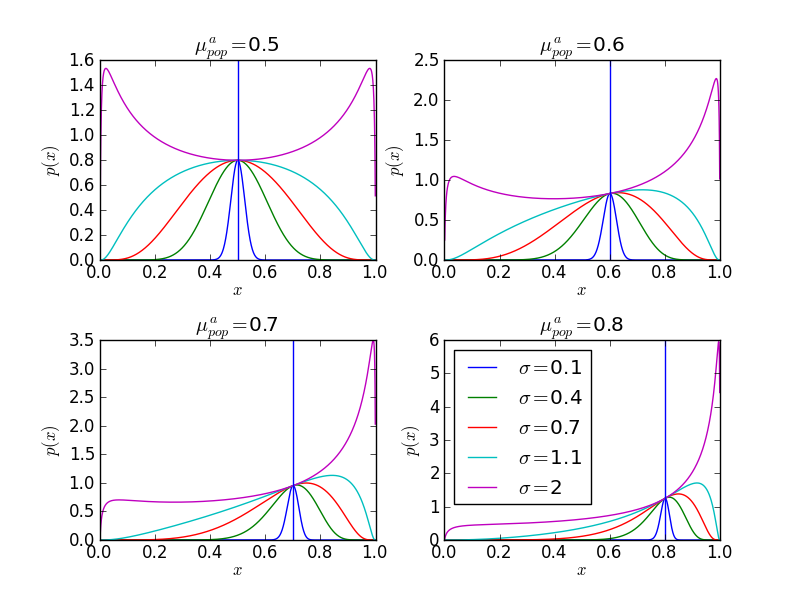
\includegraphics[width=4in, height=3in]{/Users/glareprotector/prostate_git/glare/tex_files/sections/normal_prior/files/mu_a_pdf.png}
\caption{prior predictive distribution of $\tilde{\mu}^a$}
\end{center}
\end{figure}

In Figure X, we plot how the mode of $P(\tilde{\mu}^a;c^a)$ changes with $\tilde{\sigma}^a$, as $\mu_{pop}^a$ is held fixed.  We do this for several values of $\mu_{pop}^a$.

\subsection{Choosing $c^a$ and $\lambda^a$}

We are ultimately concerned in the prior predictive distribution of $\tilde{a}$.  The previous analysis informs us that we should choose $c^a$ to ensure that $\tilde{\sigma}^a$ is less than 1 most of the time, as $mu^a$ is unimodal in those situations.  Due to our data renormalization, we can make the assumption that $\tilde{X}$ follows a multivariate $N(0,I)$ distribution.  Then, to pick $c^a$, one can follow the following steps:

\begin{enumerate}
  \item Choose a proportion $\rho$ such that you want proportion $\rho$ of possible test samples $\tilde{X}$ to have an unimodal distribution for $P(\mu^;|C^a,X)$
  \item Calculate (analytically or otherwise) the $c^a$ such that $P(\tilde{\sigma}^a < 1) = \rho$.
\end{enumerate}

Once $c^a$ is chosen, we understand the distribution $P(\mu^a;X,c^a)$.  However, what we care about is $P(a;X,c^a,\lambda^a)$.  Even if $P(\mu^a;c^a,X)$ is unimodal, $P(a;c^a,X,\lambda^a)$ may not be unimodal if $\lambda^a$ is too small.  The reason is that if $\phi^a$ is too large, the variance of $P(a;c^a,X,\lambda^a)$ will be large even if the variance of $P(\mu^a;X,c^a)$ is small, and large variances preclude unimodality of distributions.  While we cannot fix $\phi^a$ to be small, we can place a prior on $\phi^a$ that encourages it to be small.  As $\phi^a$ follows a (truncated) exponential distribution with rate parameter $\lambda^a$, the larger $\lambda^a$ is, the more likely $\phi^a$ is to be small.  Thus, we choose $\lambda^a$ finding a value such that in $P(a;c^a,X,\lambda^a)$ is unimodal most of the time.